\section*{Notes}
\addcontentsline{toc}{section}{Notes}
Due to the style of assignment my approach has been to build small code bits and
use them to solve the problem, instead of trying to build one larger program
that could only solve this specific problem.
\section*{Creating $f(x)$}
\addcontentsline{toc}{section}{Creating $f(x)$}
First part of this assignment was to create a funktion $f(x) = lovest 28bit of
(s||u)$. I have done this by shifting the bits of s right by the length of u,
and then using bitwice OR to add u on the left side. as the result is 56bit long
I used a long-type to store it for this midway calculation. Then I simply put it
through the MD5 found in Java's java.security.MessageDigest library, and use a
28bit bitmask to get nly the lovest 28 bits via bitwice AND.\\
two versions of this function can be found in EncFunc.java, as i need one for
the key, that kan take a chalenge as input, and one for the table, that can take a
key as input.

\section*{Building the RainbowTable}
\addcontentsline{toc}{section}{Building the RainbowTable}
To build the rainbow table i needed another function: $f_i(x)=(f(x) + i)$ mod
$2^{28}$ this is also implemeted in EncFunc.java.\\
The table itself is in a class RainbowTable.java, that stores in a
java.util.Hashtable, I store endpoints as keys, and the coresponding startpoints
as values. In the RainbowTable there are also two methods used to save/load the
hashtable to a file.

For the actual creation of the table I chose to stick with the suggested
chainlength / tablesize given in the assignment, I then simply loop
$[0\dots tablesize]$ pick a random startingpoint that's not in my Hashtable yet,
and run the $f_i(x)$ function on it until i reach chainlegth, with $i =
[0\dots chainlength]$. Afther that I store the starting / endingpoints, and save
the table to a file.\\
I also took statisics on my coverage in the $2^{28}$ keyspace, and got:
\FloatBarrier
\begin{figure}[h]
\centering
\makebox[\textwidth]{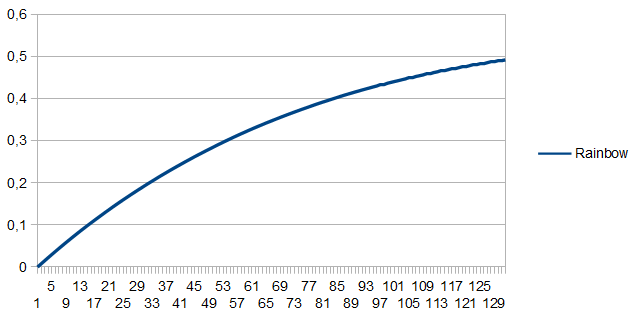
\includegraphics[width=\textwidth]{Rainbow_coverage}}
\caption{\emph{Coverage}: This RainbowTable covers roughly half the possible
keys.}
\label{fig:ClassDia}
\end{figure}
\FloatBarrier
\section*{Online: Finding the key}
\addcontentsline{toc}{section}{Online: Finding the key}
Going into the online phase I Used my preselected challenge to generate a
response from the key, using the FOBFunction() in EncFunc, I then check if the
responce exists in the table by running throug it in the pattern:
\begin{lstlisting}
for(int i = 0; i< chain; i++)
	for(int j = 0; j < i; j++)
		r = f(r, (chain - i) + j)
\end{lstlisting}
and comparing the result to the stord endPoints in my table. If I find a match i
then compute forward from the mathing startPoint until i get to the column
before the on i started at. A list of results of this can be seen in the
results.txt file.
\hyperref[appendix]{output}.
\section*{Conclusion}
\addcontentsline{toc}{section}{Conclusion}
I managed to find the exact secret i gave the FOB-key, however this seems to be
by sher luck as several repeats with different FOB-keys yielded nothing, I also
in all runs got alot of hits that lead to nowhere, I have included a results.txt
file that contains the entire output from this run.
